\documentclass{article}
\usepackage[a4paper,
total={6.5in, 10in},
voffset=5px]{geometry}
\usepackage{fancyhdr}
\usepackage[fleqn]{amsmath}
\usepackage{titling}
\usepackage[shortlabels]{enumitem}
\usepackage{amsthm}
\usepackage{amssymb}
\usepackage[bb=boondox]{mathalfa}
\usepackage{ifthen}
\usepackage{amsfonts}
\usepackage{algorithm}
\usepackage{algpseudocode}
\usepackage{indentfirst}
\usepackage{tikz}
\usepackage{tkz-graph}
\usepackage{float}
\usepackage{hyperref}
\usepackage{cleveref}
\usepackage{MnSymbol}
\usepackage{ifthen}
\usepackage{listings}
\usepackage{bussproofs}
\usepackage{lineno}
\usepackage{multicol}
\usepackage{biblatex}

\bibliography{f2}

\linenumbers

\renewcommand\linenumberfont{\normalfont\small\sffamily}
\fontfamily{qcr}\selectfont

\usetikzlibrary{positioning}

\hypersetup{
  colorlinks=true,
  allcolors=blue,
}

% \pagestyle{fancy}

\algnewcommand\algorithmicinput{\textbf{Input:}}
\algnewcommand\Input{\item[\algorithmicinput]}
\algnewcommand\algorithmicoutput{\textbf{Output:}}
\algnewcommand\Output{\item[\algorithmicoutput]}
\algnewcommand\Ret[1]{\State \textbf{return }$#1$ }
\algnewcommand\Clarif{\item[\textbf{Clarification: }]}
\algnewcommand\Assign[2]{\State $#1 = #2$}

\algnewcommand \Foreach[3]{\For{$#1 \textbf{ in } #2$}
  #3
  \EndFor
}

\algnewcommand \IIf[2]{\If{$#1$}
  #2
  \EndIf}

\algnewcommand \IIfE[3]{\If{$#1$}
  #2
  \Else
  #3
  \EndIf}

\algnewcommand \Func[3]{\Function{#1}{#2}
  #3
  \EndFunction}

\algnewcommand \Whl[2]{
  \While{$#1$}
  #2
  \EndWhile
}

\algrenewcommand\textproc{}
\newcommand{\LineComment}[1]{\\/*\textit{#1}\hfill*/}

\definecolor{codegreen}{rgb}{0,0.6,0}
\definecolor{codegray}{rgb}{0.5,0.5,0.5}
\definecolor{codepurple}{rgb}{0.58,0,0.82}
\definecolor{backcolour}{rgb}{0.95,0.95,0.92}

\lstdefinestyle{mystyle}{
    backgroundcolor=\color{backcolour},   
    commentstyle=\color{codegreen},
    keywordstyle=\color{magenta},
    numberstyle=\small\color{codegray},
    stringstyle=\color{codepurple},
    breaklines=true,                 
    captionpos=b,                    
    numbers=left,                    
    numbersep=5pt,
    showspaces=false,                
    showstringspaces=false,
    showtabs=false,                  
    tabsize=4
}
\lstset{style=mystyle}

\newcommand{\axiom}[1]{\AxiomC{$#1$}}
\newcommand{\unary}[1]{\UnaryInfC{$#1$}}
\newcommand{\binary}[1]{\BinaryInfC{$#1$}}
\newcommand{\trinary}[1]{\TrinaryInfC{$#1$}}
\newcommand{\quaternary}[1]{\QuaternaryInfC{$#1$}}
\newcommand{\rlabel}[1]{\RightLabel{#1}}

\DeclareFieldFormat{url}{\ifhyperref{\href{#1}{Link.}}{\url{#1}}}
\nocite{*}

\theoremstyle{definition}
\newtheorem{question}{Question}
\newtheorem{lemma}{Lemma}
\newtheorem{corollary}{Corollary}
\newtheorem{definition}{Definition}

\begin{document}
\pagenumbering{arabic}

Sorry that I did not communicate for last month.  The reason of that is I did not know
what to ask or not know what's missing, along with other things that distracted me.
To summarize, I was reading various papers to fill in more knowledge on DOT, and a
book \cite{lattice}.


\section{Some algebraic analysis}

The reason I started to read this book to try to understand how misbehaving DOT can be
if a bad-bound occurs. Specifically, I want to answer following question:

\begin{question}
To which point the type lattice will be jeopardized if a bad bound is accepted?
\end{question}

It turns out that, some simple lattice algebraic analysis shows the following:

\begin{lemma}
  \label{lem:collapse} Any bad bound collapses the type lattice into a single point.
\end{lemma}

This requires that bad bound involves two types whose relation we know do not look
like what bad bound says. Let me illustrate what my thought is in greater
details. This analysis is by hand so I try to be very careful about it.

First, we can form a complete lattice out of DOT's concrete types:

\begin{definition}
  \cite[2.4]{lattice} For a non-empty ordered set $P$, for all $S \subseteq P$, there
  is a supremum($\bigvee S$) and infimum($\bigwedge S$) of $S$, then $P$ is a complete
  lattice.
\end{definition}

We can define both supremum and infimum very intuitively. Then we can reason about the
lattice just by using supremum and infimum operations. The interesting part of this
theory is it tells a lot of what an equivalence class should look like without having
to specify what defines the equivalence relation, and that the ordered set is. In this
context, we only care about one equivalence relation $A =:= B$, which is implied by
$A <: B, B <: A$. We can check that it satisfies reflexivity, symmetry and
transitivity, so it's indeed an equivalence relation.

Moreover, this equivalence relation is a congruence.

\begin{definition}
  \cite[6.5]{lattice} A congruence is an equivalent relation that's compatible with
  supremum and infimum.
\end{definition}

$A =:= B$ is congruence, because it's effectively defined based on the deductive
closure of the consequence where $A =:= B$ holds. Following describes what congruences
should look like in lattices.

\begin{lemma}
  \cite[6.14]{lattice} \label{lem:sublattice} $\theta$ is a congruence on lattice $L$
  if and only if each block of $\theta$ is a sublattice of $L$.
\end{lemma}

Following is a specialization and a convenient form of argument that I use a lot when
doing reasoning.

\begin{lemma}
  \cite[6.13, 6.14]{lattice} \textbf{The quadrilateral argument: } Consider following
  diagrams, where $a \to b$ means $a \le b$ for some order relation. Bold line asserts
  some equivalence relation($\equiv$).

  \begin{figure}[H]
    \begin{multicols}{2}
      \begin{figure}[H]
        \centering
        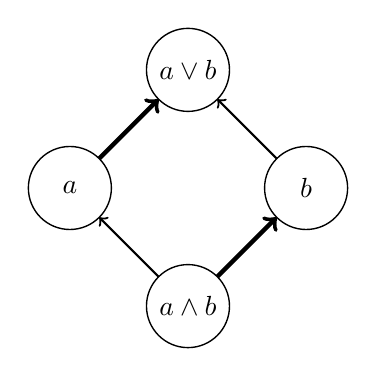
\begin{tikzpicture}
          \SetGraphUnit{1.5}
          \SetVertexMath
          \tikzset{EdgeStyle/.append style={->}}
          \tikzset{VertexStyle/.append style = {minimum size = 30pt}}

          \Vertices{circle}{b, a}

          \NOEA[L={a \vee b}](a){c}
          \SOEA[L={a \wedge b}](a){d}

          \Edge[style={ultra thick}](a)(c)
          \Edge(b)(c)
          \Edge(d)(a)
          \Edge[style={ultra thick}](d)(b)
        \end{tikzpicture}
      \end{figure}

      \begin{figure}[H]
        \centering
        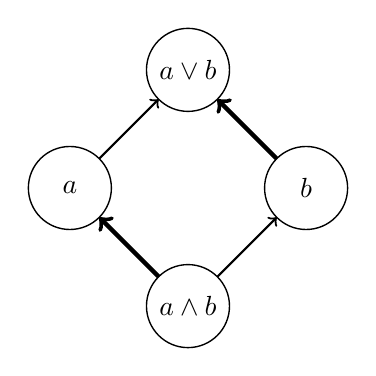
\begin{tikzpicture}
          \SetGraphUnit{1.5}
          \SetVertexMath
          \tikzset{EdgeStyle/.append style={->}}
          \tikzset{VertexStyle/.append style = {minimum size = 30pt}}

          \Vertices{circle}{b, a}

          \NOEA[L={a \vee b}](a){c}
          \SOEA[L={a \wedge b}](a){d}

          \Edge(a)(c)
          \Edge[style={ultra thick}](b)(c)
          \Edge[style={ultra thick}](d)(a)
          \Edge(d)(b)
        \end{tikzpicture}
      \end{figure}
    \end{multicols}
    \caption{quadrilateral argument}
  \end{figure}

  The argument says that any one of the pairs in the equivalence relation will force
  the other one in the pair to be also in the equivalence relation.
\end{lemma}

\begin{proof}
  It can be shown by straightforward equational reasoning. For the diagram on the
  left, if $a \equiv a \vee b$, then $a \wedge b \equiv (a \vee b) \wedge b = b$. The
  second derivation is due to $b \le a \vee b \Rightarrow a \vee b = b$. Other
  directions can be proved symmetrically.
\end{proof}

If we treat concrete types in DOT in such form, then we can apply lots of tools to
reason about it.

\begin{lemma}
Bad bound must introduce equivalences.
\end{lemma}
\begin{proof}
  There are two types of bad bound, one type is when $A <: B$, the program introduces
  $B <: A$ somehow, then in this case, we have acquired the new equivalence, so it's
  trivial in this case; the other type is when $A, B$ are not comparable, then
  $A <: B$ is asserted. We can see that this also implies equivalence relation.

  \begin{figure}[H]
    \centering
    \begin{multicols}{2}
      \begin{figure}[H]
        \centering
        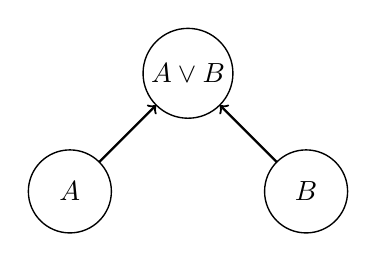
\begin{tikzpicture}
          \SetGraphUnit{1.5}
          \SetVertexMath
          \tikzset{EdgeStyle/.append style={->}}
          \tikzset{VertexStyle/.append style = {minimum size = 30pt}}

          \Vertices{circle}{B, A}

          \NOEA[L={A \vee B}](A){C}
          \Edge(A)(C)
          \Edge(B)(C)
        \end{tikzpicture}
      \end{figure}

      \begin{figure}[H]
        \centering
        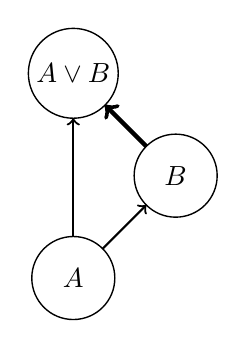
\begin{tikzpicture}
          \SetGraphUnit{1.3}
          \SetVertexMath
          \tikzset{EdgeStyle/.append style={->}}
          \tikzset{VertexStyle/.append style = {minimum size = 30pt}}

          \Vertex {A}
          \NOEA (A){B}

          \NOWE[L={A \vee B}](B){C}
          \Edge(A)(C)
          \Edge[style={ultra thick}](B)(C)
          \Edge(A)(B)
        \end{tikzpicture}
      \end{figure}    
    \end{multicols}
    \caption{bad bound between two irrelevant types}
  \end{figure}
  
  The left shows the original relation. Since DOT forms complete lattice, we know
  $A \vee B$ exists; when we force $A <: B$, we turn left into diagram on the
  right. Then, it asserts that $A \vee B =:= B$. Since we assumed that $A, B$ are not
  comparable, we know $A \vee B =:= B$ originally does not hold, hence a new
  equivalence.
\end{proof}

Therefore, we know that whenever bad bound occurs, we must have introduced new
equivalence relation somehow. However, attention needs to be paid here by actually
defining what a bad bound is. We call a bound bad, because it ``makes no sense''. To
spell it out, both sides of the bound already have certain relation that we know
(either subtype relation or no relation), which contradicts to what the bad bound
says. In that sense, it's clearly that we won't call the following program introduces
a bad bound:

\nolinenumbers
\begin{lstlisting}[language=Haskell, mathescape=true]
  $\mu$ x : {
    A : x.B .. x.C
    B : x.C .. x.A
    C : x.A .. x.B
  }
\end{lstlisting}
\linenumbers

Because path types are, intuitively, not considered ``concrete'', therefore it has
freedom to be whatever it is. In another word, if a bad bound occurs, we are saying
that some two concrete types. Having this in mind, we can see how bad bound behaves by
proving the claim (\cref{lem:collapse}) in the beginning.

\begin{proof}
  We have four kinds of concrete types, $\top$, $\bot$, objects and functions. Any
  equivalence relation can involve any pair of them. We have 8 non-trivial cases, and
  following can be easily discharged: $\top =:= \bot$, object $=:=$ functions.

  The case for collapsing $\top$ and objects is very general. Consider following
  quadrilateral argument ($F$ is any function type):
  
  \begin{figure}[H]
    \centering
    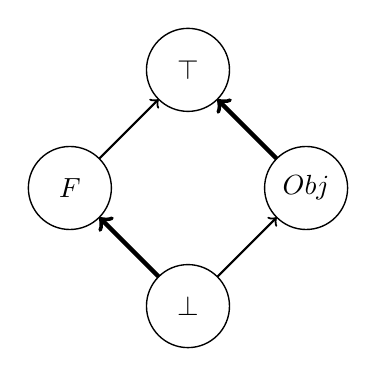
\begin{tikzpicture}
      \SetGraphUnit{1.5}
      \SetVertexMath
      \tikzset{EdgeStyle/.append style={->}}
      \tikzset{VertexStyle/.append style = {minimum size = 30pt}}

      \Vertices{circle}{Obj, F}

      \NOWE[L={\top}](Obj){C}
      \SOWE[L={\bot}](Obj){D}
      \Edge(F)(C)
      \Edge[style={ultra thick}](Obj)(C)
      \Edge[style={ultra thick}](D)(F)
      \Edge(D)(Obj)
    \end{tikzpicture}
    \caption{quadrilateral argument for function and object types}
  \end{figure}

  This holds because all functions are incomparable with any object. Therefore their
  supremum and infimum must be $\top$ and $\bot$ respectively. Now applying
  quadrilateral argument shows $F$ and $\bot$ must collapse. Note that $F$ is not
  specified, therefore it applies for all function types. By transitivity of
  equivalence relation, all function types become equivalent. Specifically,
  $\forall(x: \top)\top$ and $\forall(x: \top)\bot$ collapse, which implies $\top$ and
  $\bot$ also collapse.

  This pattern is very general. Due to the incomparability between function types and
  object types, we can show that if any one of them collapse with either $\top$ or
  $\bot$, then we can infer $\top$ and $\bot$ also collapse. This rules out following
  cases: $\top =:=$ object, $\top =:=$ function, $\bot =:=$ object, $\bot =:=$
  function.

  We have only two cases left, function collapse with function and object with
  object. The former introduces two smaller equivalent relation, and therefore can be
  dischargable by induction.

  Then what's left is to show that collapsing two different objects implies the
  diagram above. But it's not difficult. There are only two relations between two
  objects: either one is subtype of another, or they are not comparable, which are
  captured by following quadrilateral arguments:

  \begin{figure}[H]
    \begin{multicols}{2}
      \begin{figure}[H]
        \centering
        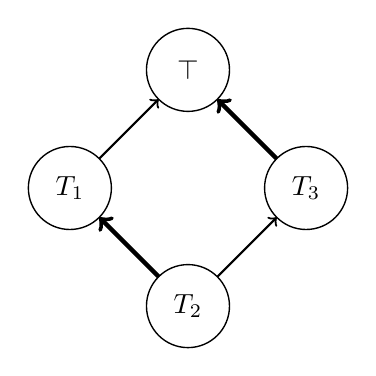
\begin{tikzpicture}
          \SetGraphUnit{1.5}
          \SetVertexMath
          \tikzset{EdgeStyle/.append style={->}}
          \tikzset{VertexStyle/.append style = {minimum size = 30pt}}

          \Vertices{circle}{T_3, T_1}

          \NOWE[L={\top}](T_3){C}
          \SOWE[L=T_2](T_3){D}
          \Edge(T_1)(C)
          \Edge[style={ultra thick}](T_3)(C)
          \Edge[style={ultra thick}](D)(T_1)
          \Edge(D)(T_3)
        \end{tikzpicture}
      \end{figure}
      
      \begin{figure}[H]
        \centering
        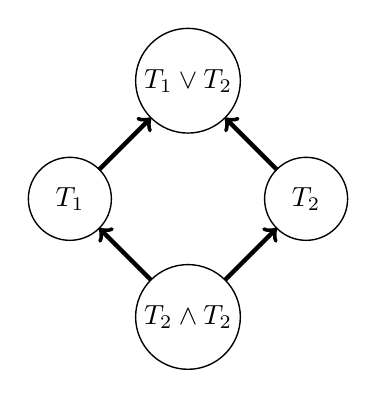
\begin{tikzpicture}
          \SetGraphUnit{1.5}
          \SetVertexMath
          \tikzset{EdgeStyle/.append style={->}}
          \tikzset{VertexStyle/.append style = {minimum size = 30pt}}

          \Vertices{circle}{T_2, T_1}

          \NOWE[L={T_1 \vee T_2}](T_2){C}
          \SOWE[L={T_2 \wedge T_2}](T_2){D}
          \Edge[style={ultra thick}](T_1)(C)
          \Edge[style={ultra thick}](T_2)(C)
          \Edge[style={ultra thick}](D)(T_1)
          \Edge[style={ultra thick}](D)(T_2)
        \end{tikzpicture}
      \end{figure}
    \end{multicols}
    \caption{object $=:=$ object}
  \end{figure}
  
  Consider the first case. If we know $T_2 <: T_1$, then we know for those fields they
  intersect, they must either be the same, or possess some proper subtyping relation.
  We can split two cases according to this, either there are at least one fields in
  both $T_1, T_2$ such that one in $T_2$ is a further refinement of one in $T_1$; or
  $T_2$ must have fields that do not exist in $T_1$, and we can aggregate those fields
  in $T_3$. Following are example of each case:

  \nolinenumbers
  \begin{multicols}{2}
    \begin{lstlisting}[language=Haskell, mathescape=true]
$T_1$ := $\mu$ x : {
  A : $\bot$ .. $\top$
}
    \end{lstlisting}

    \begin{lstlisting}[language=Haskell, mathescape=true]
$T_2$ := $\mu$ x : {
  A : $\bot$ .. { $\mu$ y : { AA : $\bot$ .. $\top$ } }
  B : $\bot$ .. $\top$
}
    \end{lstlisting}
  \end{multicols}    
  \linenumbers

  We can see that $A$ is refined, so we can only $T_2 <: T_1$; while in the case where
  such refinement does not occur, it's captured by the left diagram above:

  \nolinenumbers
  \begin{multicols}{2}
    \begin{lstlisting}[language=Haskell, mathescape=true]
$T_1$ := $\mu$ x : {
  A : $\bot$ .. $\top$
}
    \end{lstlisting}

    \begin{lstlisting}[language=Haskell, mathescape=true]
$T_2$ := $\mu$ x : {
  A : $\bot$ .. $\top$
  B : $\bot$ .. $\top$
}
    \end{lstlisting}
  \end{multicols}    
  \linenumbers

  The latter case has shown that $T_3 =:= \top$ just like the diagram on the left. For
  the former case, then there must be at least one fields that is refined in $T_2$ and
  the reason for the bad bound. This then can be discharged by induction to find out
  what's the type equivalent to $\top$ or $\bot$.
  
  For the other diagram, if we assert $T_1 =:= T_2$, then by \cref{lem:sublattice},
  the smallest sublattice must be in the same equivalence class. Specifically, we can
  derive $T_1 \wedge T_2 =:= T_1 \vee T_2$ and they cannot be the same, assuming
  $T_1 =:= T_2$ is introduced by bad bound. If $T_1 \vee T_2$ is $\top$ then we are
  done; otherwise, we fall back to the previous case, and we've learned that there
  must be another type that becomes equivalent to one of the extrema.

  We've exhausted all the cases at this point, and the original claim is proved.
\end{proof}

\cref{lem:collapse} is very helpful, it basically says if there is indeed a lattice
structure in the type system, then we can conclude the following:

\begin{corollary}
  With bad bound's presence, all terms can be typed to $\bot$. 
\end{corollary}

So this treatment of bad bounds is very tempting. It matches what intuition says: once
we detect a bad bound, which is determined to not being able to instantiate, why
bother typing the program under its influence in the first place? $\bot$, then,
becomes a flag that says ``following program is nonsense''. From algebra, there seems
to be a clearer track on what can be done to make typing easier. So my question is
following,

\begin{question}
Do you know any similar algebraic analysis done on calculi with subtyping?
\end{question}

However, the current DOT does not have this structure. From algebraic perspective, it
seems to show the current definition has following problems:

\begin{enumerate}
\item In above discussion, I implicitly fit all objects into a sublattice. This does
  not work in current DOT, due to each recursive type form its own little blob. I was
  mentioning to change this, which will be discussed below.
  
\item The intersection types introduces lots of equivalent types that are
  syntactically not the same. For example, in above argument, If $F \wedge Obj \neq
  \bot$, then the proof breaks, and it's what happens in DOT. $F \wedge Obj$ has its
  own right to be a type in DOT, except that it cannot be instantiated, and
  consequently it becomes a bottom that is less bottom.
  
\item Intersection type is also not quite consistent. In the case of record types,
  intersection type functions like a supremum, while not quite the case for any other
  types. The problem here is the intersection type becomes a part of the syntax,
  instead of a computation. 
\end{enumerate}

To interpret it from another side, we can say that we want to make the types in DOT to
form a well studied structure such that certain analysis can be done ``for free''. I
think these suggest that removing intersection type from type primitive and unifying
object types are good moves, which are what I am doing.

\section{Modifying DOT}

Besides removing intersection, I changed DOT's types as following:

\vspace{-15px}
\begin{align*}
  T :=&\ ...\ \text{// $\top, \bot$ function and selection remain the same. } \\
  | &\ \mu(x : DS) \\
  DS :=&\ [D] \ |\ D :: DS \\
  D :=&\ ...\ \text{// declarations as before}
\end{align*}

It effectively turns the declarations into a list that has at least one element. The
typing rule for this is routine. The subtyping rules are following:

\nolinenumbers
\begin{prooftree}
  \axiom{\Gamma, x: \mu(x: \{ a : T\} :: DS) \vdash T <: U}
  \rlabel{\textbf{(OBJ-FIELD)}}
  \unary{\Gamma \vdash \mu(x: \{ a : T\} :: DS) <: \mu(x: \{ a : U\} :: DS) }
\end{prooftree}

\begin{prooftree}
  \axiom{\Gamma, x: \mu(x: \{ A : S_1 .. T_1 \} :: DS) \vdash S_2 <: S_1}
  \axiom{\Gamma, x: \mu(x: \{ A : S_1 .. T_1 \} :: DS) \vdash T_1 <: T_2}
  \rlabel{\textbf{(OBJ-TYPE)}}
  \binary{\Gamma \vdash \mu(x: \{ A : S_1 .. T_1 \} :: DS) <: \mu(x: \{ A : S_2 .. T_2
    \} :: DS) }
\end{prooftree}
\linenumbers

Both \textbf{OBJ-FIELD, OBJ-TYPE} need straightforward variations for $[D]$.

\nolinenumbers
\begin{prooftree}
  \axiom{}
  \rlabel{\textbf{(OBJ-DROP1)}}
  \unary{\Gamma \vdash \mu(x : DS_1 ++ DS_2) <: \mu(x : DS_2) }
\end{prooftree}

\begin{prooftree}
  \axiom{}
  \rlabel{\textbf{(OBJ-DROP2)}}
  \unary{\Gamma \vdash \mu(x : DS_1 ++ DS_2) <: \mu(x : DS_1) }
\end{prooftree}

\begin{prooftree}
  \axiom{\Gamma \vdash \mu(x: DS) <: \mu(x : DS_1)}
  \axiom{\Gamma \vdash \mu(x: DS) <: \mu(x : DS_2)}
  \rlabel{\textbf{(OBJ-MERGE)}}
  \binary{\Gamma \vdash \mu(x: DS) <: \mu(x: DS_1 ++ DS_2) }
\end{prooftree}

\begin{multicols}{2}
  \begin{prooftree}
    \axiom{\Gamma \vdash x: \mu(x : \{ A : S .. T \} :: DS)}
    \rlabel{\textbf{(SEL1)}}
    \unary{\Gamma \vdash x.A <: T }
  \end{prooftree}

  \begin{prooftree}
    \axiom{\Gamma \vdash x: \mu(x : \{ A : S .. T \} :: DS)}
    \rlabel{\textbf{(SEL2)}}
    \unary{\Gamma \vdash S <: x.A }
  \end{prooftree}
\end{multicols}
\linenumbers

 Currently the rules are still not deterministic, specifically transitivity is still
around. Hopefully these rules are enough to replace the rules for original
intersection types. I originally thought that proving soundness could be easy, by
simply translating both terms and types from the modified version to the original
one, but it's not true. This modification has changed the type lattice entirely, so
the language expressed by this language is not the same one anymore. Therefore proving
it sound is basically working out another new calculus. I won't expect it to be at the
same level of difficulty, though, since \textbf{REC-I, REC-E} are removed
completely. So my question on this part is,

\begin{question}
  Should I go ahead and prove this calculus sound?
\end{question}

Notice that, this modification does not necessary jeopardize the expressiveness of the
language too badly by taking away intersection type from user level. In fact, one
observation is, as long as we can express a type being subtypes of two different types
in covariant position, we are automatically talking about intersection type. For
example,

\nolinenumbers
\begin{lstlisting}[language=Haskell, mathescape=true]
$\mu$ x : {
  A : $\bot$ .. $\top$
  B : $\bot$ .. $\top$
  C : $\bot$ .. A
  D : C .. B
}
\end{lstlisting}
\linenumbers

This has forced $C <: A \wedge D <: A \wedge B$ without spelling it out. It's the same
case for union type, whenever we have the ability to talk about relation in
contravariant position, we are forced to reason about union type, without having to
have language support. Therefore to some extent, this language looks nicer than DOT
from different angles, except that some functionality requires more verbose encoding. 

However, this language alone seem to lack power to manipulate path types, because we
can't explicitly require path type intersecting with some other types. But then this
suggests we cannot do it without explicitly defining intersection type and union type,
for the sake of dealing with path types, while in the case of no involvement of path
types, we eagerly compute the supremum and infimum. Then this suggests another
calculus, which possess rules of following kind:

\begin{prooftree}
  \axiom{\Gamma \vdash T <: S_1}
  \axiom{\Gamma \vdash T <: S_2}
  \rlabel{\textbf{(INFIMUM)}}
  \binary{\Gamma \vdash T <: infimum(S_1, S_2) }
\end{prooftree}

In this case, infimum involving path types must use intersection type:

\nolinenumbers
\begin{lstlisting}[language=Haskell, mathescape=true]
infimum x.T x.T = x.T
infimum x.T S = x.T $\wedge$ S
infimum T x.S = T $\wedge$ x.S
...
\end{lstlisting}
\linenumbers

and others similarly. Infimum and supremum computations will be widely spread out in
the typing and subtyping rules.

There seems two potential directions to go, hence the question above. The first one is
definitely going to be easier to work with, but it's unclear to me where these two
paths can lead to.

I will proceed with the first one for now. Let me know if you think it's not a good
idea.

\section{Conclusion}

I think I will keep looking into lattice theory as I found it very fruitful. I still
have a number of papers on DOT to read. I wasn't able to get too much from dotty a
while ago, but now I developed some theoretic basis, so hopefully for a second time I
can get some juice from it.

Please let me know what do you think about it and your suggestions.

\printbibliography

\end{document}